% !TeX root = ../../main.tex
% Add the above to each chapter to make compiling the PDF easier in some editors.

\section{Interactive Segmentation}\label{ord:ch2:sec3}

Image segmentation takes as input $\textbf{x}$ only the image itself.
In contrast, interactive segmentation takes beside the image some additional information interactively provided by a user.
This additional information is especially beneficial, because it is manually picked by the valuable image processing capabilities of a human.
Therefore, interactive segmentation networks are provided with high level guidance on the object of interest.
This makes interactive segmentation especially suitable to label images on pixel level.
Depending on the type of user interaction the interactive method may be more or less elaborate.
This leads to a fundamental difficulty of interactive methods, because user interaction is considered to time elaborate and therefore expensive.

The interactive segmentation of an instance may be interpreted as semantic segmentation with two classes: the foreground object to segment and the background.
In order to segment multiple objects in an image, multiple applications of these interactive methods are required.
% TODO scope of interactive segmentation here, the class is assigned manually?
In the following the principles of interactive segmentation concepts are introduced, on which the methods used in the benchmark study are built on.

\subsection{Classical Concepts}\label{ord:ch2:sec3:subsec1}
Before the emergence of \gls{dl} and \glspl{cnn}, segmentation was already performed with classical image processing.
These methods also focus on the extraction of a foreground object from the background by little user interaction.

% GraphCut and GrabCut
Prominent algorithms are Graph Cut \cite{BJ01-GraphCut} and GrabCut \cite{RKB04-GrabCut}.
As user interaction GrabCut requires a loose bounding box and optionally defining explicit image parts as fore- or background.
%Everything outside the bounding box and the borders itself are defined as background, while the inside of the box is segmented based on contrast and color information.
%Further, the goodness of the result may be enhanced by iteratively defining explicit image parts as fore- or background.

% Watershed
Another still relevant method to perform instance segmentation is the watershed transformation \cite{VS91-Watershed}.
This method interactively collects fore- and background markers from users in order to perform segmentation.
The watershed method is part of the benchmark study and elaborately examined in Section \ref{ord:ch3:sec2}.

% TODO decide if superpixel shoudl stay or not???
% Superpixels
% Last, an algorithm using so-called \textit{Superpixels} was introduced in 2003 \cite{RM03-Superpixel}.
% Superpixels are groups of connected pixels, that share similarities in color or low-level features as contour, brightness or texture.
% Further, these Superpixels are used to perform segmentation.
% This algorithms is still a current research topic, an overview of several state-of-the-ar approaches is given in \cite{SHL16-SuperpixelEvaluation}.
 
% Final thought
Although, these algorithms are based on classical image processing, they remain relevant in modern problem and research topics.


\subsection{DL User Point Concepts}\label{ord:ch2:sec3:subsec2}

\subsubsection{Basic Concept}
% DL focus 
Modern interactive segmentation algorithms combine \gls{dl} models and additional user input.
As \gls{dl} models usually \glspl{cnn} for image segmentation are applied.
% Obtaining points on fore- and background
User point centered concepts obtain the user input in the form of clicks on the image.
The user clicks are often differentiated between clicks on the foreground object and clicks on the background.
The input $\textbf{x}$ of an interactive segmentation network is a combination of the image and the user clicks.

This fundamental concept is used for various interactive segmentation models \cite{Xu16-InteractiveObjectSelection} \cite{MVL18-ITIS} and exemplary shown in Figure \ref{fig:ch2:sec3:ifcn}
% IOG and DEXTR explained in detail in following chapter.
Further, the methods \gls{dextr}  \cite{Man18-DEXTR} and \gls{iog} \cite{Zha20-IOG} also follow a user point centered concept. They are part of the benchmark study and extensively described in Section \ref{ord:ch3:sec3} and \ref{ord:ch3:sec4}.

Interactive segmentation networks are often based on normal segmentation networks, \eg the \gls{fcn} in the \gls{ifcn} \cite{Xu16-InteractiveObjectSelection} or the DeepLabv3+ in the \gls{itis} network \cite{MVL18-ITIS}.
As for segmentation networks, the prediction $\hat{y}$ of interactive networks is a probability map.

\begin{figure}
	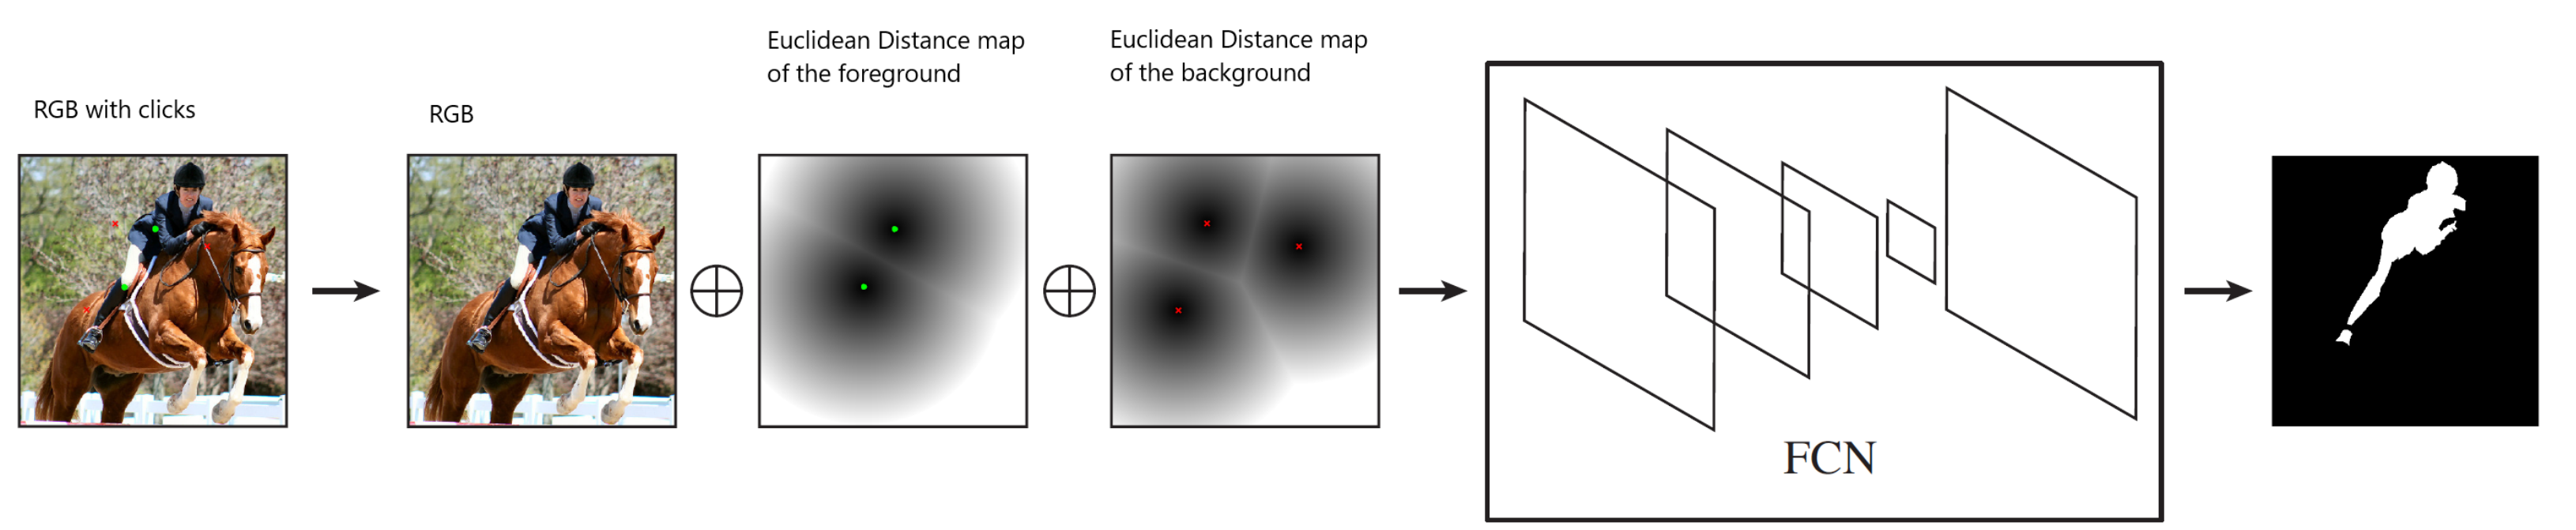
\includegraphics[width=\linewidth]{figures/chap232_ifcn.png}
	\caption[Interactively Fully Convolutional Network]{
		Illustration of the pipeline from the \gls{ifcn}.
		The input is a \gls{rgb} image with user clicks.
		This input is displayed in its individual parts as \gls{rgb}, map of the fore- and background points.
		The network in use is based on the \gls{fcn} and outputs a binary segmentation result.
		Copyright \copyright 2016 IEEE. Reprinted by permission from \cite{Xu16-InteractiveObjectSelection}
	}\label{fig:ch2:sec3:ifcn}
\end{figure}

\subsubsection{Representation of User Clicks and Model Input}
The user clicks are transformed into points on heatmaps, that have the same spacial dimension as the input image.
In order to distinguish between fore- and background points, there exist separate heatmaps for fore- and background.
In some literature the foreground points are also called \textit{positive} points, while the background points are called \textit{negative} points.
If there is only one type of points, there also exists only one heatmap.

% Modification of points -> gauss or euclidean
The heatmaps are further processed, in order to highlight the set user points.
This may be achieved by the conversion into an Euclidean distance map \cite{Dan80-EuclideanDistanceMapping} (see Figure \ref{fig:ch2:sec3:ifcn}) or the application of a Gauss filter.
Thereby, the a Gauss filter leads to slightly better results the Euclidean distance map, as examined in \cite{Man18-DEXTR} and \cite{MVL18-ITIS}.

% TODO  Evtl. könnte man auch damit argumentieren, dass damit die Ungenauigkeit der User-Clicks adressiert wird und man vermeiden will, dass man nur ein binäres, sehr sparses Signal an das Modell übergibt. Wäre eigentlich mal eine interessante Ablation study ob es wirklich notwendig ist diese Gauß-Anwendung durchzuführen.

% 3 RGB Channels + 2 Heatmaps = 5-Channel input
The image is usually colored with the three \gls{rgb} channels.
The heatmaps have the same size as the image and are concatenated to the image as additional channels.
%This results in a five- or four-channel input for the interactive segmentation network, depending on the number of heatmaps.
This results in a five-channel input using fore-and background heatmaps or in a four-channel input using just a foreground heatmap.
Many methods \cite{Man18-DEXTR} \cite{Zha20-IOG} crop the image and heatmaps based on the user points and then process only the reduced input, in order to direct the focus on the object of interest.

The processed points on the heatmaps and the user clicks on the image are located exactly at the same position on different channels.
This matching is vital for the functionality of the segmentation method.
The user points provide high level guidance for the network to enhance the location and differentiation of fore- and background.
The multidimensional input is used as model input $\textbf{x}$ for the semantic segmentation network.


\subsubsection{Interactive Refinement}
A fundamental advantage of interactive methods is the presence of a human user.
The interactive segmentation network may not always deliver a satisfactory result in the initial execution.
In this case, interactive methods often provide the option to refine the initial result.
In order to apply the refinement, the user sets an additional click on the fore- or background region, where the segmentation fails.
This refinement click is added to the corresponding heatmap and the network is executed again based on the updated input.
This refinement process may be applied iteratively by the user and thereby also enforces guidance on the object to segment.
Further, interactive refinement specifically focuses on regions of failure, while other models without user interaction must rely on their initial predictions.


\subsubsection{Characteristics}
% Similar to normal segmentation networks.
Interactive segmentation networks have similar characteristics as normal segmentation networks.
For training they require the multidimensional input $\textbf{x}$, while the label $y$ is just the mask from the object of interest.
Interactive segmentation methods usually aims at segmenting an object, which represents the foreground, from the background.
This results in a class-agnostic problem with the two classes fore- and background, while semantic segmentation distinguishes between several classes.

% Simulation of user clicks.
To create a suitable input $\textbf{x}$ for training, the user clicks are regularly simulated, which requires that the corresponding \gls{gt} is available.
Simulations are compulsory to create the associated user clicks for complete datasets, because it would be too expensive and inconsistent if the user clicks of whole datasets were created by real users.
Therefore, also the evaluation of trained interactive segmentation methods is mostly based on simulations, due to their advantages in scalability, costs, and time.
However, it should be noted that simulations cannot fully mimic real users and therefore have certain drawbacks as discussed in Section \ref{ord:ch5:sec_3_generalization_user}.

% Refinement Training
The training setup for iterative refinement is more elaborate.
The refinement clicks are simulated online during the training process.
In the simulation the refinement clicks are usually set within the largest areas that are predicted wrongly.
This is calculated based on the \gls{gt} and the prediction $\hat{y}$ of the previous model execution.

\subsubsection{Variations}
% Special Methods 
%    - Iterative learning
%    - Fusion networks
While the presented concept is the most common approach and achieves state-of-the-art results, there are other mentionable ideas and variations:
\begin{itemize}
	% One click
	\item \textbf{One-Click Segmentation} is introduced in \cite{Maj20-One-Click} and this networks requires only one foreground click per object.
	%This click is processed as foreground click and enforced with a Gauss filter.
	This foreground click is enforced with a Gauss filter and the segmentation is based on the DeepLab network.
	This method used the most simple form of user interaction.
	However, it cannot reach the performance of state-of-the-art networks.
	
	\item The \textbf{\gls{fctsfn}} stands out, due to the separate processing of image and user clicks \cite{Hu19-TwoStreamFusionNetwork}.
	% The fore- and background points are converted into two feature maps, that contain an Euclidean distance map.
	The user clicks and the image are processed separately by two streams.
	These two processing streams share the same architecture based on VGG16, but have their own weights.
	The intent is to learn the deep features from image and user clicks individually.
	Last, the two streams are combined and processed together to create one prediction.
	Nevertheless, \gls{fctsfn} is outperformed by other methods as shown in Table \ref{tab:ch2:interactive-stae-of-the-art}.
	
	\item \textbf{Iterative training} is applied in the \gls{itis} network \cite{MVL18-ITIS}.
	Every epoch a new refinement click is added to the multidimensional input.
	This click is simulated during the training process, based on the classification result of the previous epoch.
	It is claimed, that this novel \textit{iterative training procedure} significantly improves the networks performance.
	While \gls{itis} requires on average less clicks to reach a \gls{miou} of 85\%, other methods perform better with four at four clicks (see Table \ref{tab:ch2:interactive-stae-of-the-art}).
	
\end{itemize}


\subsubsection{Evaluation and State-of-the-Art Networks} \label{ch2:sec3:eval_interactive_methods}
% Describe Evaluation metrics: clicks requried for certain iou and iou at certain amount of clicks
For a reliable evaluation of interactive methods the user interaction has to be taken into account.
For user interactions based on clicks, two metrics are widely used together, represented in Table \ref{tab:ch2:interactive-stae-of-the-art}. 
The first metric lists the number or clicks, that a model requires to achieve a certain level of accuracy. 
The number of clicks must not be an integer, due to the averaging of all results of the dataset.
The second metric lists the model's accuracy for a certain amount of clicks.

% Limitations.
However, these types of evaluation metric reach their limits, addressed in the following:
The first metric is actually only applicable if a method has the possibility to perform a refinement.
The second metric does not always enable a fair comparison, because for various methods the underlying functionality may be different. 
For example, the minimal required amount of clicks may be lower or higher than the amount of clicks, which is set for comparison.

% Problems with the evaluation of time.
For interactive methods, the time required for the user interaction is fundamental for the application, because as many images as possible should be labeled as quickly as possible.
Since a uniform setup is not given, the measured times of single papers are not comparable.
% TODO Den Satz, dass nicht klar ist wie lange man für einen Klick braucht (und dass das von Methode zu Methode unterschiedlich schwer ist) könnte man auch weiter vor ziehen. Ein Beispiel, dass etwa in DEXTR möglichst genau der Rand getroffen werden muss, bei IOG aber nur grob die Mitte des Objekts wäre auch hilfreich für den Leser. Dann wird sofort klar was damit gemeint ist.
% The measured time by single papers is not comparable, due to the missing of a common setup to perform uniform user studies for these novel methods.
With these metrics the time is only approximated by the number of clicks.
But these metrics do not include indicators that describe how much effort it takes to set a click and how much time it takes.
Further, there is no common metric to evaluate the usability of these interactive methods.

Nevertheless, these metrics are currently the preferred method to evaluate interactive segmentation methods.
They are still suitable to compare interactive segmentation models in a meaningful way, but with the mentioned limitations.

A comparison of several referred methods and the current state-of-the-art methods is given in Table \ref{tab:ch2:interactive-stae-of-the-art}.


% State of the art
\begin{table}[h!]
	\centering
	\begin{tabular}{l|c|c}
		\textbf{Model} 	& \textbf{Number of clicks} & \textbf{mIoU (\%) @ 4 clicks} \\
						& PASCAL VOC @ 85\% mIoU 	& PASCAL VOC \\
		\hline
		% TODO add watersheds if available for PASCAL VOC
		Graph Cut \cite{BJ01-GraphCut}									  & > 20 & 41.1\\
		\glsentryshort{ifcn} \cite{Xu16-InteractiveObjectSelection}       & 6.9  & 75.2\\
		\glsentryshort{risnet} \cite{Liew17-RegionalInteractiveImageSeg}  & 5.7  & 80.7\\
		\glsentryshort{itis} \cite{MVL18-ITIS}			 				  & 3.4  & 86.9\\
		\glsentryshort{fctsfn} \cite{Hu19-TwoStreamFusionNetwork}		  & 4.6  & 82.2\\
	    \glsentryshort{dextr} \cite{Man18-DEXTR} 	     				  & 4    & 91.5\\
		\glsentryshort{iog} \cite{Zha20-IOG}	 	    				  & 3    & 94.4\\
	\end{tabular}
	\caption[Comparison of interactive segmentation models.]{
		Comparison of interactive segmentation models on the PASCAL \gls{voc} 2012 test set with application of the \gls{vp}.
		It can be seen, that interactive segmentation methods have developed quickly. 
		They strongly improved in terms of required clicks and \gls{iou}.
		% TODO ?? PASCAL \gls{voc} is at its limit to be suitable to evaluate semantic segmentation.
	} \label{tab:ch2:interactive-stae-of-the-art}
\end{table}

\subsection{\gls{dl} Polygon Concepts}\label{ord:ch2:sec3:subsec3}
This concept is based on the idea to use a \gls{dl} model to predict a polygon.
The polygon itself aim to represent the border of the segmentation mask, while the inside of the polygon represents the mask.

The following is a brief summary of the method represented in \cite{Ling19-Curve-GCN}.
% Workflow + UI
As initial user interaction a loose bounding box around the object of interest is required.
Based on this box the image is cropped and the crop is used as model input.

% Architecture
The \gls{dl} model consists out of a combination of several subnetworks and architectural components.
First, the cropped image is inputted into a \gls{cnn}, which provides the extracted features and a boundary prediction to the third component.
Second, a fixed size polygon is initialized, to transform the task into a graph problem.
Third, a multi-layer \gls{gcn} iteratively shifts the position of each polygon node towards the object boundary. 
This method is named \textit{Curve-\gls{gcn}}, inspired by the \textit{curved} approximation of a closed polygon.
% Good user interaction - refinement
The user is able to perform refinement, by interactively moving single nodes of the polygon.
% Performance
% The performance of the \textit{Curve-\gls{gcn}} is only represented on the Cityscapes Dataset, but it claim to perform 
Details of this method can be reviewed in \cite{Ling19-Curve-GCN}.
In experiments on datasets as CityScapes or Rooftop the \textit{Curve-\gls{gcn}} is outperformed by the \gls{iog} method, which is presented in Section \ref{ord:ch3:sec4}.

% Vorreiter von Curve GCN \cite{Acu18-Polygon-RNN++}
The predecessor of the \textit{Curve-\gls{gcn}} is based on \glspl{rnn} and introduced in \cite{Acu18-Polygon-RNN++}.





